\bluepage{Rendering Pipeline / Zobrazovací řetězec}

\begin{frame}
\frametitle{GPU / Rendering Pipeline / Zobrazovací řetězec}
  \scriptsize
	\begin{itemize}
		\item GPU is divided into memory and rendering pipeline.
	\end{itemize}
	\begin{itemize}
		\item GPU je rozděleno na paměť a vykreslovací řetěžec.
	\end{itemize}
	\begin{picture}(320,250)
		\put(0,100){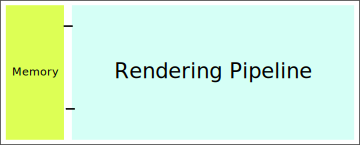
\includegraphics[width=12.5cm,keepaspectratio]{pics/pipeline/RenderingPipelineMemoryPipeline}}
	\end{picture}
\end{frame}

\begin{frame}
\frametitle{Rendering Pipeline / Zobrazovací řetězec}
  \scriptsize
	\begin{itemize}
		\item Rendering Pipeline is divided into 2 parts: vector and raster.
    \item Splitting element is rasterization.
	\end{itemize}
	\begin{itemize}
		\item Zobrazovací řetěžec je rozdělen na 2 části - vektorovou a rastrovou.
    \item Dělícím prvkem je rasterizace.
	\end{itemize}
	\begin{picture}(320,250)
		\put(0,100){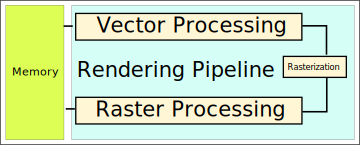
\includegraphics[width=12.5cm,keepaspectratio]{pics/pipeline/RenderingPipelineVectorRaster}}
	\end{picture}
\end{frame}

\begin{frame}
\frametitle{Vector Part / Vektorová část}
  \scriptsize
	\begin{itemize}
		\item The main goal of vector part is to transform geometry.
    \item It processes vertices, primitives, it performs transformations, clipping, cullling, tessellation, projection,...
	\end{itemize}

	\begin{itemize}
		\item Hlavním úkolem vektorové části je transformace geometrie.
    \item Počítá vertex, primitiva, provádí transformace, ořez, teselaci, projekci, ...
	\end{itemize}

	\begin{picture}(320,250)
		\put(0,100){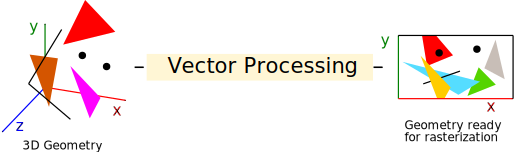
\includegraphics[width=12.5cm,keepaspectratio]{pics/pipeline/pipeline_vector_overview}}
	\end{picture}
\end{frame}

\begin{frame}
\frametitle{Rasterization / Rasterizace}
  \scriptsize
	\begin{itemize}
    \item The goal of rasterization is to convert vector graphics elements (triangles, lines, points) to fragments.
	\end{itemize}

	\begin{itemize}
    \item Cílem rasterizace je převod vektorových grafických elementů (trojúhelníky, čáry, body) na fragmenty.
  \end{itemize}
	\begin{picture}(320,250)
		\put(0,100){
\includegraphics[width=12.5cm,keepaspectratio]{pics/pipeline/rasterization_overview}}
	\end{picture}
\end{frame}

\begin{frame}
\frametitle{Raster Part / Rastrová část}
  \scriptsize
	\begin{itemize}
		\item The main goal of raster part is to process fragments.
    \item It colors fragment, performs per fragment operations, depth test, stencil test, blending, ...
	\end{itemize}

	\begin{itemize}
		\item Hlavním úkolem rastrové části je výpočet fragmentů.
    \item Obarvuje fragment, provádí per fragment operace, hloubkový test, stencil test, blending, ...
	\end{itemize}
	\begin{picture}(320,250)
		\put(0,100){
\includegraphics[width=12.5cm,keepaspectratio]{pics/pipeline/pfo_overview}}
	\end{picture}
\end{frame}


\begin{frame}
\frametitle{Vector Part / Vektorová část}
  \scriptsize
	\begin{itemize}
		\item Vector Part is composed of many blocks.
    \item Some of the blocks are programable, some can be skipped.
	\end{itemize}
	\begin{itemize}
		\item Vektorová část řetězce je složena z mnoha bloků.
    \item Některé bloky jsou programovatelné a některé vynechatelné.
	\end{itemize}
	\begin{picture}(320,250)
		\put(0,60){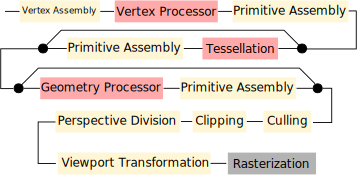
\includegraphics[width=12.5cm,keepaspectratio]{pics/pipeline/RenderingPipelineVector}}
	\end{picture}
\end{frame}

\begin{frame}
\frametitle{Zlednodušená Vektorová část}
  \scriptsize
	\begin{itemize}
		\item If we remove optional blocks, the pipeline looks like this.
	\end{itemize}
	\begin{itemize}
		\item Pokud vynecháme volitelné bloky, zůstane zjednodušená vektorová část řetězce.
	\end{itemize}
	\begin{picture}(320,250)
		\put(0,60){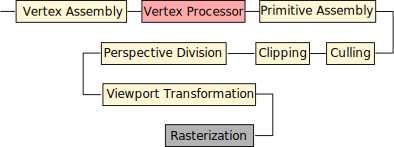
\includegraphics[width=12.5cm,keepaspectratio]{pics/pipeline/simplified_pipeline}}
	\end{picture}
\end{frame}

\begin{frame}
\frametitle{Vertex Assembly, vertex processor, primitive assembly}
  \scriptsize
	\begin{itemize}
		\item Vertex Assembly creates vertices.
    \item Vertex processor transforms vertices.
    \item Primitive assembly creates base primitives from transformed vertices.
  \end{itemize}
	\begin{itemize}
		\item Vertex Assembly sestavuje vrcholy
    \item Vertex processor transformuje vrcholy
    \item Primitive assembly sestavuje základní primitiva.
	\end{itemize}
	\begin{picture}(320,250)
		\put(0,100){
\includegraphics[width=12.5cm,keepaspectratio]{pics/pipeline/OpenGL460PipelineVertexShader}}
	\end{picture}
\end{frame}

\begin{frame}
\frametitle{Vertex, Vertex Assembly}
  \scriptsize
	\begin{itemize}
		\item Vertex is a structure of vertex attributes.
    \item Vertex Assembly unit reads data from memory and forms vertices.
	\end{itemize}

	\begin{itemize}
		\item Vertex je struktura vertex atributů
    \item Vertex Assembly jednotka se stará o sestavování vrcholů z bufferů.
	\end{itemize}
	\begin{picture}(120,150)
		\put(0,0){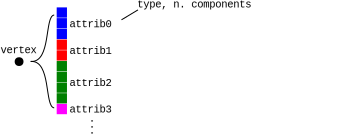
\includegraphics[width=12.5cm,keepaspectratio]{pics/pipeline/vertex}}
	\end{picture}
	\begin{picture}(60,40)
		\put(50,0){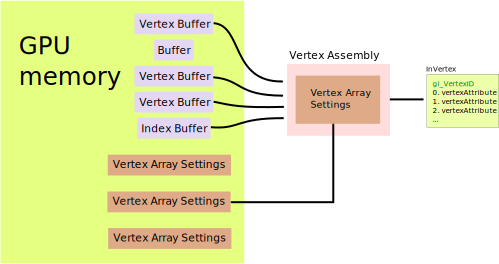
\includegraphics[width=8cm,keepaspectratio]{pics/pipeline/vertexAssembly}}
	\end{picture}
\end{frame}

\begin{frame}
\frametitle{Vertex Assembly - indexované kreslení}
  \scriptsize
	\begin{itemize}
		\item Vertex Assembly can utilize indexing
    \item Vertex Cache - already processed vertices do not have to be processed again
	\end{itemize}
	\begin{itemize}
		\item Vertex Assembly může využít indexování
    \item Vertex Cache - jednou propočítané vrcholy není třeba počítat znovu
	\end{itemize}
	\begin{picture}(120,150)
		\put(25,0){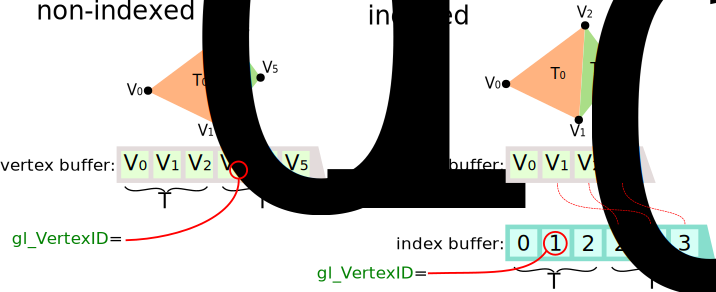
\includegraphics[width=12.5cm,keepaspectratio]{pics/pipeline/drawElements}}
	\end{picture}
\end{frame}

\begin{frame}
\frametitle{Vertex Processor}
	\begin{itemize}
		\item Ve Vertex Processoru běží vertex shader.
    \item Vertex Shader je uživatelem specifikovaný program.
    \item Cílem je transformovat vstupní vrchol na výstupní vrchol.
	\end{itemize}
	\begin{picture}(120,150)
		\put(25,0){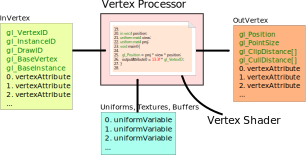
\includegraphics[width=10.5cm,keepaspectratio]{pics/pipeline/vertexShader}}
	\end{picture}
\end{frame}

\begin{frame}
\frametitle{Primitive Assembly}
	\begin{itemize}
		\item Primitive Assembly jednotka sestavuje primitiva.
    \item Cílem je podle nastavení sestavovat trojúhelníky, úsečky, vrcholy.
    \item Základní primitiva (trojúhleník, úsečka) mohou být součástí složitějších primitive.
    \item Triangle Strip, Triangle Fan, Line Strip, Triangle Adjacency, Patch, ...
	\end{itemize}
	\begin{picture}(120,150)
		\put(25,0){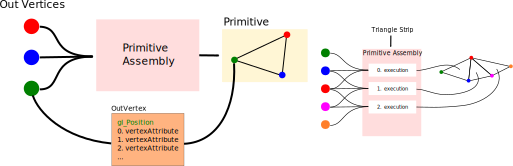
\includegraphics[width=8.5cm,keepaspectratio]{pics/pipeline/PrimitiveAssembly}}
	\end{picture}
\end{frame}

\begin{frame}
\frametitle{Culling, clipping}
	\begin{itemize}
		\item Těsně před raterizací se zahazují odvrácené trojúhelníky a zbylé se ořezávají pohledovým frustem.
	\end{itemize}
	\begin{picture}(320,250)
		\put(0,100){
\includegraphics[width=12.5cm,keepaspectratio]{pics/pipeline/OpenGL460PipelineClipping}}
	\end{picture}
\end{frame}

\begin{frame}
\frametitle{Culling}
	\begin{itemize}
		\item Culling se stará o zahazování odvrácených trojúhelníků.
    \item Odvrácenost je rozhodnuta na základě pořadí vrcholů.
    \item Je možné nastavit, jestli je trojúhelník přivrácený nebo odvrácený, pokud jsou vrcholy po nebo proti směru hodinových ručiček.
	\end{itemize}
	\begin{picture}(120,150)
		\put(25,25){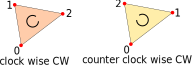
\includegraphics[width=8.5cm,keepaspectratio]{pics/pipeline/culling}}
	\end{picture}
\end{frame}

\begin{frame}
\frametitle{Clipping, near-plane clipping}
	\begin{itemize}
		\item Pokud je primitivum jen částečně uvnitř pohledového jehlanu, je potřeba jej oříznout.
    \item Obvykle stačí oříznout pomocí blízké ořezové roviny (near-plane).
    \item Pokud vznikne čtyčúhelník, je možné jej nahradit dvěma trojúhelníky.
	\end{itemize}
	\begin{picture}(120,150)
		\put(0,0){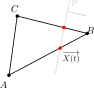
\includegraphics[width=4.5cm,keepaspectratio]{pics/pipeline/clip}}
	\end{picture}
	\begin{picture}(60,40)
		\put(25,0){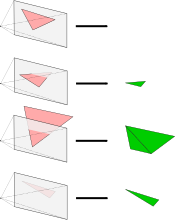
\includegraphics[width=4cm,keepaspectratio]{pics/pipeline/clip_variants}}
	\end{picture}
\end{frame}

\begin{frame}
\frametitle{Perspektivní dělení}
	\begin{itemize}
		\item Blok perspektivního dělení převádí homogenní souřadnice na kartézské.
    \item Dělí se pomocí W, ve kterém je uložena hloubka. Tím se zmenšují objekty, které jsou dál od kamera.
    \item Po perspekvitním dělení všechny vrcholy leží v rozsahu $[-1,+1]$ - normalized device coordinates.
	\end{itemize}
	\begin{picture}(120,150)
		\put(50,0){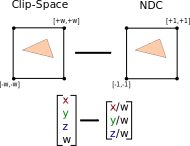
\includegraphics[width=6.5cm,keepaspectratio]{pics/pipeline/PerspectiveDivision}}
	\end{picture}
\end{frame}

\begin{frame}
\frametitle{Viewport transformace}
	\begin{itemize}
		\item Blok viewport transformace transformuje normalizované souřadnice na rozlišení plátna.
	\end{itemize}
	\begin{picture}(120,150)
		\put(50,0){
\includegraphics[width=8.5cm,keepaspectratio]{pics/pipeline/ViewportTransformation}}
	\end{picture}
\end{frame}

\begin{frame}
\frametitle{Teselace}
	\begin{itemize}
		\item Tesselace je složena zde 2 programovatelných processorů a hardwarového generátoru primitiv.
	\end{itemize}
	\begin{picture}(320,250)
		\put(0,100){
\includegraphics[width=12.5cm,keepaspectratio]{pics/pipeline/OpenGL460PipelineTessellationShaders}}
	\end{picture}
\end{frame}

\begin{frame}
\frametitle{Geometry processor, transform feedback}
	\begin{itemize}
		\item Geometry processor transformuje primitiva.
    \item Transform feedback může primitiva přeposlat zpět do bufferu.
	\end{itemize}
	\begin{picture}(320,250)
		\put(0,100){
\includegraphics[width=12.5cm,keepaspectratio]{pics/pipeline/OpenGL460PipelineGeometryShader}}
	\end{picture}
\end{frame}

\begin{frame}
\frametitle{Rasterizace}
	\begin{itemize}
		\item Rasterizace produkuje fragmenty.
    \item Fragment je datová struktura, která vznikne na pozici vzorku (sampling point).
    \item Vzorkovací bod je obvykle uprostřed pixelu.
    \item Situace je komplikovanější při využití multi-samplingu.
    \item Pokud leží vzorkovací bod uvnitř trojúhelníku, vznikne fragment pro daný pixel.
	\end{itemize}
	\begin{figure}[h]
		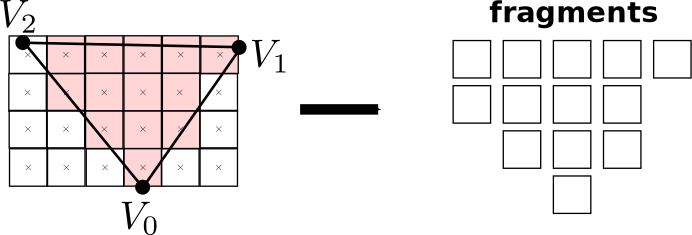
\includegraphics[width=10cm,keepaspectratio]{pics/pipeline/rasterization.pdf}
	\end{figure}
\end{frame}

\begin{frame}
\frametitle{Rasterizace a interpolace}
	\begin{itemize}
		\item Vertexy jsou před rasterizací popsány pomocí n-tice atributů
    \item Rasterizace produkuje fragmenty, pokud jejich střed leží uvnitř primitiva
    \item Po rasterizaci jsou tyto atributy vloženy do fragmetů pomocí interpolace
	\end{itemize}
	\begin{figure}[h]
		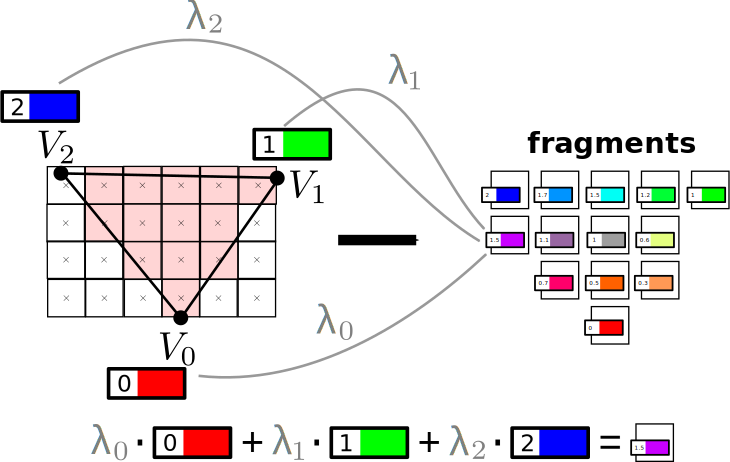
\includegraphics[width=10cm,keepaspectratio]{pics/pipeline/interpolation.pdf}
	\end{figure}
\end{frame}

\begin{frame}
\frametitle{Barycentrické koordináty}
	\begin{figure}[h]
		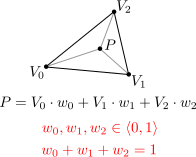
\includegraphics[width=8cm,keepaspectratio]{pics/pipeline/barycentrickekoordinaty.pdf}
	\end{figure}
\end{frame}

\begin{frame}
\frametitle{Barycentrické koordináty ve 2D}
	\begin{figure}[h]
		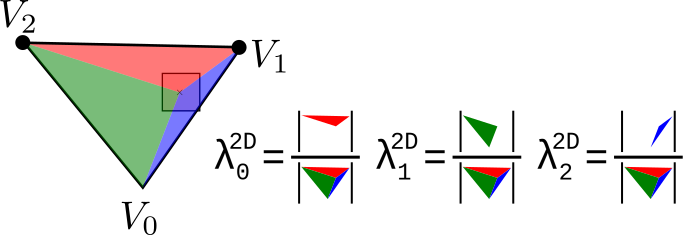
\includegraphics[width=8cm,keepaspectratio]{pics/pipeline/barycentric2D.pdf}
	\end{figure}
\end{frame}

\begin{frame}
\frametitle{Perspektivní zkreslení}
	\begin{itemize}
		\item Vertex atributy se mohou interpolovat v rovině průmětny nebo v prostoru scény
    \item Aby se mohlo interpolovat v prostoru scény, musí se provést perspektivní korekce
      (v OpenGL automaticky/lze vypnout)
	\end{itemize}
	\begin{figure}[h]
		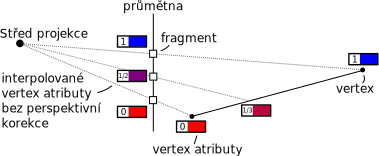
\includegraphics[width=10cm,keepaspectratio]{pics/pipeline/prespektivni_korekce.pdf}
	\end{figure}
\end{frame}

\begin{frame}
\frametitle{Fragment Processor}
	\begin{itemize}
		\item Ve Fragment Processoru běží fragment shader.
    \item Fragment Shader je uživatelem specifikovaný program.
    \item Cílem je transformovat vstupní fragment na výstupní fragment.
    \item Multiple Render Target.
	\end{itemize}
	\begin{figure}[h]
		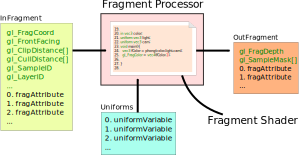
\includegraphics[width=8cm,keepaspectratio]{pics/pipeline/FragmentShader.pdf}
	\end{figure}
\end{frame}

\begin{frame}
\frametitle{Rastrová část - Brzké testy a operace}
	\begin{picture}(320,250)
		\put(0,20){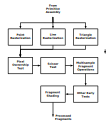
\includegraphics[width=7cm,keepaspectratio]{pics/pipeline/OpenGL460PipelineRaster}}
	\end{picture}
\end{frame}

\begin{frame}
\frametitle{Rastrová část - Pozdní testy a Per fragment operace}
	\begin{picture}(320,250)
		\put(-20,20){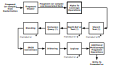
\includegraphics[width=12.5cm,keepaspectratio]{pics/pipeline/OpenGL460PipelineFragmentShader}}
	\end{picture}
\end{frame}

\begin{frame}
\frametitle{PFO - depth test}
	\begin{picture}(320,250)
		\put(50,30){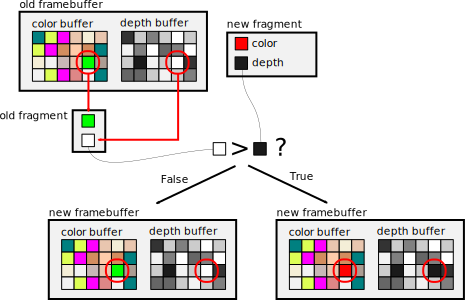
\includegraphics[width=10.5cm,keepaspectratio]{pics/pipeline/PFO}}
	\end{picture}
\end{frame}


\begin{frame}
\frametitle{OpenGL 4.6 pipeline}
  \begin{figure}[h]
  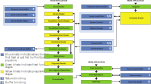
\includegraphics[width=10cm,keepaspectratio]{pics/pipeline/OpenGL460Pipeline}
  \end{figure}
\end{frame}


